En el presente capítulo se explica la experimentación 
realizada para la clasificación de los videos del 
\textit{dataset Hockey Fights}. La 
estructura que se detalla a continuación consiste de: 
explicación del \textit{pipeline}, la experimentación 
con las diferentes configuraciones de BI-LSTM y la 
comparativa de los resultados.

\section{Pipeline propuesto}

La Imagen \ref{metodologia} ilustra la metodología propuesta, 
la cual se procederá a explicar a continuación:

\begin{figure}[h!] 
    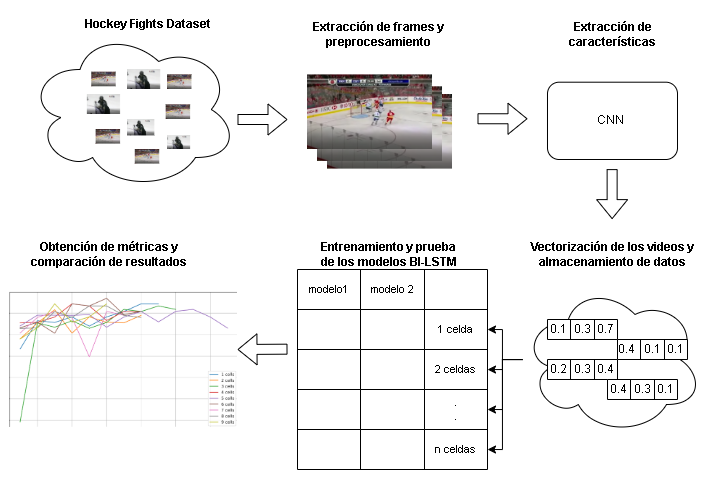
\includegraphics[width=0.7\textwidth]{images/metodologiaMaestria.png} 
    \centering 
    \caption{Metodología propuesta. Creación propia.} 
    \label{metodologia} 
\end{figure}

El \textit{pipeline} consiste en la obtencion, preprocesamiento 
y almacenamiento de las caracteristicas obtenidas del 
\textit{dataset}, para luego ser pasado a las diferentes 
configuraciones de los modelos BI-LSTM, los cuales se 
encargarán cada video basado en sus frames y finalmente 
se evaluarán los resultados basados en la métrica f1 y 
el tiempo de inferencia.

\subsection{Extracción de frames y preprocesamiento}

Como primer paso de la metodología se necesitó realizar un 
preprocesamiento de los datos para su análisis posterior a 
través de los modelos mencionados en el anterior capítulo. 
Como primer paso, se procedió a descargar el 
\textit{dataset} a través de su repositorio de 
\href{https://www.kaggle.com/datasets/yassershrief/hockey-fight-vidoes/data}{Kaggle}. \\

Una vez obtenidos los datos, se procedió a etiquetar cada uno 
de los videos basados en los nombres de cada uno de ellos. 
Se puede diferenciar su etiqueta debido a que aquellos que 
comiencen con "fi" contienen violencia, mientra que los demás, 
no. Con los videos cargados, se recolectaron los frames tal 
como fue mencionado anteriormente. Para ello, se decidió 
hacer un muestreo de 10 frames de manera equitativamente 
separada del video (1 por cada 4 frames). Cada uno de estos 
frames fueron redimensionados a un formato estandar (224 x 224) 
para luego ser normalizados.

\subsection{Obtención de las características}

Con cada conjunto de frames por video, estos pasan a través de 
las diferentes arquitecturas de CNN mencionadas en el anterior 
capítulo. Para ello, se tuvieron las siguientes consideraciones: 
\begin{itemize}
    \item Se obtendrán los modelos pre-entrenados con el 
    dataset ImageNet.
    \item Se eliminan las capas de clasificación.
    \item Se agrega una capa GlobalAveragePooling2D para 
    reducir la dimensionalidad de kernels(resultado de las CNN). 
    \item Se marca al modelo final como no entrenable.
\end{itemize}
 
Este ultimo paso es necesario debido a que se utilizará el 
conocimiento pre-entrenado de los modelos para obtener 
únicamente el vector característico de cada una de las 
imágenes. En ese sentido, se hace innecesario el proceso de 
entrenamiento de estas. Además, sería contraproducente tanto 
entrenar una CNN basado únicamente en frames porque pueden 
existir casos en el que existen frames donde no hay violencia 
y viceversa y también debido a que se perdería parte del 
conocimiento que ya tienen estos modelos. Finalemente se 
procedió a guardar estos vectores de características en 
formato h5. \\

Cabe resaltar que en la realidad podría implementarse un 
modelo conjunto con la CNN y LSTM, pero algunos de los modelos 
(especialmente los EfficientNet) contienen capas que no son 
facilmente mapeables a las entradas de las BI-LSTM, por lo 
cual se tuvo que hacer esto como  preprocesamiento.

\subsection{Entrenamiento y prueba del clasificador}

Como clasificador, se tuvo un modelo de BI-LSTM con diferente 
número de celdas. Para esta experimentación, se decidió usar 
un número entre 1 y 9 celdas, ya que consistía en un dataset 
bastante sencillo y altamente estudiado anteriormente. 

Para cada uno de las CNN's mencionadas en la anterior sección, 
y para cada una de las configuraciones, se procedió a 
entrenar y testear cada combinación de ellas. Las consideraciones 
para esta arquitectura fueron las siguientes:

\begin{itemize}
    \item De entrada se tienen los vectores de características 
    obtenidos del paso anterior (se debe considerar que los 
    tamaños de salida puden variar con respecto a la CNN). 
    \item Se crea un modelo BI-LSTM con X celdas, 10 timesteps 
    (en otras palabras los 10 frames obtenidos) y el tamaño 
    del output del anterior paso.
    \item Capas densas de 1024, 50 y 2 neuronas con funciones 
    de activación RelU y la última de tipo softmax. 
    \item Función de pérdida Binary CrossEntropy, optimizador adam 
    y de métricas accuracy y f1-score.
    \item Función de early stopping con \textit{patience} de 3 y  
    \textit{min delta} de 0.005 y batch de 16 videos por vez.
\end{itemize}

En la siguiente sección se presentarán los resultados 
generados utilizando las anteriores consideraciones para 
cada uno de los modelos mencionados.

\section{Experimentación}

Como primer paso, se procedió a realizar el pre-procesamiento 
de las imágenes y la obtención de sus características tal 
como fue mencionado anteriormente. Para ello, se recolectaron 
las métricas acerca de la cantidad de parámetros y el 
tiempo de cálculo de cada uno de los modelos, los cuales 
se puden observar en la Tabla \ref{tabla:procesamiento}:

\begin{table}[h!]
\centering
\begin{tabular}{|l|r|r|}
\hline
\multicolumn{1}{|c|}{\textbf{Modelo}} & \multicolumn{1}{c|}{\textbf{Parámetros}} & \multicolumn{1}{c|}{\textbf{\begin{tabular}[c]{@{}c@{}}Timpo de inferencia\\ (por batch de 10)\\ en ms/batch\end{tabular}}} \\ \hline
\textbf{efficientnetb0}               & 4,049,571                                & 46 ms                                                                                                                       \\ \hline
\textbf{resnet50}                     & 23,587,712                               & 51 ms                                                                                                                       \\ \hline
\textbf{efficientnetv2-s}             & 20,331,360                               & 75 ms                                                                                                                       \\ \hline
\textbf{MobilenetV3large}             & 2,996,352                                & 45 ms                                                                                                                       \\ \hline
\end{tabular}
\label{tabla:preprocesamiento}
\end{table}

Se puede apreciar que el tamaño final de los modelos fue 
menor que el esperado por la Tabla \ref{evaluación}. 
Esto se debió a que no se están utilizando las capas densas 
de los modelos y se estan reemplazando con una capa 
GlobalAveragePooling2D, la cual obtiene el resultado del 
kernel final de las capas convolucioanles y las reduce a un 
solo resultado promediado. 

Habiendo obtenido las características de cada uno de las 
imágenes y los diez frames generados por cada uno de ellas, 
se entrenaron diferentes modelos BI-LSTM como fue mencionado 
anteriormente, teniendo desde 1 a 10 celdas para cada uno de 
los CNN utilizados. A continuación se muestran las gráficas 
de pérdida y f1 score para cada una de los experimentos. 

\begin{figure}[h!]
    \centering
    \subfloat[\centering F1 score por época]{\includegraphics[width=0.48\textwidth]{../graphs/efficientnetb0_val_loss_per_epoch.png}}
    \subfloat[\centering Pérdida por época]{\includegraphics[width=0.48\textwidth]{../graphs/efficientnetb0_val_f1_per_epoch.png}}\hfill
    \caption{Gráficos de pérdida y f1 score por época usando EfficientNetB0}
    \label{fig:combinedEfficientnetB0}
\end{figure}

\begin{figure}[h!]
    \centering
    \subfloat[\centering F1 score por época]{\includegraphics[width=0.48\textwidth]{../graphs/efficientnetv2-s_val_loss_per_epoch.png}}
    \subfloat[\centering Pérdida por época]{\includegraphics[width=0.48\textwidth]{../graphs/efficientnetv2-s_val_f1_per_epoch.png}}\hfill
    \caption{Gráficos de pérdida y f1 score por época usando EfficinetnetV2-S}
    \label{fig:combinedEfficientnetV2}
\end{figure}


\begin{figure}[h!]
    \centering
    \subfloat[\centering F1 score por época]{\includegraphics[width=0.48\textwidth]{../graphs/MobilenetV3large_val_loss_per_epoch.png}}
    \subfloat[\centering Pérdida por época]{\includegraphics[width=0.48\textwidth]{../graphs/MobilenetV3large_val_f1_per_epoch.png}}\hfill
    \caption{Gráficos de pérdida y f1 score por época usando MobilenetV3}
    \label{fig:MobilenetV3}
\end{figure}


\begin{figure}[h!]
    \centering
    \subfloat[\centering F1 score por época]{\includegraphics[width=0.48\textwidth]{../graphs/resnet50_val_loss_per_epoch.png}}
    \subfloat[\centering Pérdida por época]{\includegraphics[width=0.48\textwidth]{../graphs/resnet50_val_f1_per_epoch.png}}\hfill
    \caption{Gráficos de pérdida y f1 score por época usando Resnet50}
    \label{fig:Resnet50}
\end{figure}

